%aaaaaaaaaaaaaaaaaaaaaaaaaaaaaaaaaa
%This is the LaTeX ARTICLE template for RSC journals
%Copyright The Royal Society of Chemistry 2014
%%%%%%%%%%%%%%%%%%%%%%%%%%%%%%%%%%%
\documentclass[twoside,twocolumn,9pt]{article}
\usepackage{extsizes}
\usepackage[super,sort&compress,comma]{natbib} 
\usepackage[version=3]{mhchem}
\usepackage[left=1.5cm, right=1.5cm, top=1.785cm, bottom=2.0cm]{geometry}
\usepackage{balance}
\usepackage{widetext}  
\usepackage{times,mathptmx}
\usepackage{sectsty}
\usepackage{graphicx} 
\usepackage{lastpage}
\usepackage[format=plain,justification=raggedright,singlelinecheck=false,font={stretch=1.125,small,sf},labelfont=bf,labelsep=space]{caption}
\usepackage{float}
\usepackage{fancyhdr}
\usepackage{upgreek}
% \usepackage{fnpos}
\usepackage[english]{babel}
\usepackage{array}
% \usepackage{droidsans}
\usepackage{charter}
\usepackage[T1]{fontenc}
\usepackage[usenames,dvipsnames]{xcolor}
\usepackage{setspace}
\usepackage[compact]{titlesec}
%%%Please don't disable any packages in the preamble, as this may cause the template to display incorrectly.%%%

\usepackage[sf,SF]{subfigure}
\usepackage{multirow}

\usepackage{ulem}

%\usepackage{epstopdf}%This line makes .eps figures into .pdf - please comment out if not required.

\definecolor{cream}{RGB}{222,217,201}

\begin{document}

\pagestyle{fancy}
\thispagestyle{plain}
\fancypagestyle{plain}{

%%%HEADER%%%
\fancyhead[C]{\includegraphics[width=18.5cm]{head_foot/header_bar}}
\fancyhead[L]{\hspace{0cm}\vspace{1.5cm}\includegraphics[height=30pt]{head_foot/journal_name}}
\fancyhead[R]{\hspace{0cm}\vspace{1.7cm}\includegraphics[height=55pt]{head_foot/RSC_LOGO_CMYK}}
\renewcommand{\headrulewidth}{0pt}
}
%%%END OF HEADER%%%

%%%PAGE SETUP - Please do not change any commands within this section%%%
\makeFNbottom
\makeatletter
\renewcommand\LARGE{\@setfontsize\LARGE{15pt}{17}}
\renewcommand\Large{\@setfontsize\Large{12pt}{14}}
\renewcommand\large{\@setfontsize\large{10pt}{12}}
\renewcommand\footnotesize{\@setfontsize\footnotesize{7pt}{10}}
\makeatother

\renewcommand{\thefootnote}{\fnsymbol{footnote}}
\renewcommand\footnoterule{\vspace*{1pt}% 
\color{cream}\hrule width 3.5in height 0.4pt \color{black}\vspace*{5pt}} 
\setcounter{secnumdepth}{5}

\makeatletter 
\renewcommand\@biblabel[1]{#1}            
\renewcommand\@makefntext[1]% 
{\noindent\makebox[0pt][r]{\@thefnmark\,}#1}
\makeatother 
\renewcommand{\figurename}{\small{Fig.}~}
\sectionfont{\sffamily\Large}
\subsectionfont{\normalsize}
\subsubsectionfont{\bf}
\setstretch{1.125} %In particular, please do not alter this line.
\setlength{\skip\footins}{0.8cm}
\setlength{\footnotesep}{0.25cm}
\setlength{\jot}{10pt}
\titlespacing*{\section}{0pt}{4pt}{4pt}
\titlespacing*{\subsection}{0pt}{15pt}{1pt}
%%%END OF PAGE SETUP%%%

%%%FOOTER%%%
\fancyfoot{}
\fancyfoot[LO,RE]{\vspace{-7.1pt}\includegraphics[height=9pt]{head_foot/LF}}
\fancyfoot[CO]{\vspace{-7.1pt}\hspace{13.2cm}\includegraphics{head_foot/RF}}
\fancyfoot[CE]{\vspace{-7.2pt}\hspace{-14.2cm}\includegraphics{head_foot/RF}}
\fancyfoot[RO]{\footnotesize{\sffamily{1--\pageref{LastPage} ~\textbar  \hspace{2pt}\thepage}}}
\fancyfoot[LE]{\footnotesize{\sffamily{\thepage~\textbar\hspace{3.45cm} 1--\pageref{LastPage}}}}
\fancyhead{}
\renewcommand{\headrulewidth}{0pt} 
\renewcommand{\footrulewidth}{0pt}
\setlength{\arrayrulewidth}{1pt}
\setlength{\columnsep}{6.5mm}
\setlength\bibsep{1pt}
%%%END OF FOOTER%%%

%%%FIGURE SETUP - please do not change any commands within this section%%%
\makeatletter 
\newlength{\figrulesep} 
\setlength{\figrulesep}{0.5\textfloatsep} 

\newcommand{\topfigrule}{\vspace*{-1pt}% 
\noindent{\color{cream}\rule[-\figrulesep]{\columnwidth}{1.5pt}} }

\newcommand{\botfigrule}{\vspace*{-2pt}% 
\noindent{\color{cream}\rule[\figrulesep]{\columnwidth}{1.5pt}} }

\newcommand{\dblfigrule}{\vspace*{-1pt}% 
\noindent{\color{cream}\rule[-\figrulesep]{\textwidth}{1.5pt}} }

\makeatother
%%%END OF FIGURE SETUP%%%

%%%TITLE, AUTHORS AND ABSTRACT%%%
\twocolumn[
  \begin{@twocolumnfalse}
\vspace{3cm}
\sffamily
\begin{tabular}{m{4.5cm} p{13.5cm} }

\includegraphics{head_foot/DOI} & \noindent\LARGE{\textbf{Water Dissociative Adsorption on $\alpha$-Al$_{\text{2}}$O$_{\text{3}}$(11\=20) is Controlled by Surface Site Undercoordination, Density and Topology$^\dag$}} \\%Article title goes here instead of the text "This is the title"
\vspace{0.3cm} & \vspace{0.3cm} \\

 & \noindent\large{Sophia Heiden,\textit{$^{a}$} Yanhua Yue,\textit{$^{b}$} Harald Kirsch,\textit{$^{b}$} Jonas Wirth,\textit{$^{a}$} Peter Saalfrank,\textit{$^{a}$} and R.\ Kramer Campen$^{\ast}$\textit{$^{b}$}} \\%Author names go here instead of "Full name", etc.

\includegraphics{head_foot/dates} & \noindent\normalsize{$\alpha$-\ce{Al2O3} surfaces are common in a wide variety of applications and useful models of more complicated, environmentally abundant, alumino-silicate surfaces. While several decades of work have clarified that all properties of these surfaces depend sensitively on crystal face and the presence of even small amounts of water, quantitative insight into this dependence has proven challenging. Overcoming this challenge requires systematic study of the {\it mechanism} by which water interacts with various $\alpha$-\ce{Al2O3} surfaces. Such insight is most easily gained for the interaction of small amounts of water with surfaces in UHV. In this study we continue our combined theoretical and experimental approach to this problem, previously applied to water interaction with the $\alpha$-\ce{Al2O3} (0001) and (1\=102) surfaces, to water interaction with the third most stable surface, \textit{i.e.}\ the (11\=20). Because we characterize all three surfaces using similar tools, it is straightforward to conclude that the (11\=20) is most reactive with water. The most important factor explaining its increased reactivity is that the high density of undercoordinated surface Al atoms on the (11\=20) surface allow the bidentate adsorption of OH fragments originating from dissociatively adsorbed water while only monodentate adsorption is possible on the (0001) and (1\=102) surfaces: the reactivity of $\alpha$-\ce{Al2O3} surfaces with water depends strongly, and nonlinearly, on the density of undercoordinated surface Al atoms.
} \\%The abstrast goes here instead of the text "The abstract should be..."

\end{tabular}

 \end{@twocolumnfalse} \vspace{0.6cm}

  ]
%%%END OF TITLE, AUTHORS AND ABSTRACT%%%

%%%FONT SETUP - please do not change any commands within this section
\renewcommand*\rmdefault{bch}\normalfont\upshape
\rmfamily
\section*{}
\vspace{-1cm}


%%%FOOTNOTES%%%

\footnotetext{\textit{$^{a}$~University of Potsdam, Institute of Chemistry, Karl-Liebknecht-Stra{\ss}e 24-25, 14476 Potsdam, Germany}}
\footnotetext{\textit{$^{b}$~Fritz Haber Institute of the Max Planck Society, Faradayweg 4-6, 14195 Berlin, Germany. }}

%Please use \dag to cite the ESI in the main text of the article.
%If you article does not have ESI please remove the the \dag symbol from the title and the footnotetext below.
\footnotetext{\dag~Electronic Supplementary Information (ESI) available: details of sample preparation, TPD and LEED results, VSF data analysis, review of theory of orientational dependence of VSF signal, and calculated reaction paths for single and multi-step H diffusion. See DOI: 10.1039/b000000x/}
%additional addresses can be cited as above using the lower-case letters, c, d, e... If all authors are from the same address, no letter is required

%\footnotetext{\ddag Current address of Jonas...}


%%%END OF FOOTNOTES%%%

%%%MAIN TEXT%%%%
\section{Introduction}
\label{sec1}
$\alpha$-\ce{Al2O3} surfaces are omnipresent in applications and useful models for more environmentally abundant alumino-silicate surfaces. As a result of this ubiquity they have been studied for decades using a variety of experimental and theoretical approaches\cite{brow99,eng00,Trainor02,Brown01,hass98,hass00, morterra1996case, kelb07}. This work makes clear that surface reactivity, polarity and stability all vary dramatically between $\alpha$-\ce{Al2O3} crystal face and in the presence of even small amounts of water \cite{ago2005aligned, ishigami2008crystal}. Because most engineered and all environmentally relevant $\alpha$-\ce{Al2O3} systems contain at least small amounts of water, it is clear that quantitative understanding of these heterogeneous chemical processes requires understanding how $\alpha$-\ce{Al2O3} surfaces interact with water. Standard treatments of these topics typically invoke bond valence arguments from Pauling that are common in coordination chemistry: the reactivity of a particular $\alpha$-\ce{Al2O3} surface with respect to water is a function of the degree of underbonding of its surface metal and oxygen atoms and their density \cite{pau29,hie91,stu96}. 

The vast majority of prior experimental and theoretical studies have been carried out on the most stable $\alpha$-Al$_{2}$O$_{3}$ crystal face: the (0001)\cite{hass98,nels98,toof98,hass00,Niu00,kelb07,Rane08,Rane09,zhan08,floe08,Wipp10,Wirth12,kirsch2014,tong2015optically}. Taken as a whole this work suggests that under Ultra High Vacuum (UHV) conditions this surface has one (of two possible) Al-terminations while under ambient conditions or in contact with liquid water, more complicated, oxygen terminated structures are thermodynamically favoured. The second and third most stable crystal terminations, the (1\=102) and (11\=20) surfaces respectively, are substantially less studied. However, in contrast to the (0001) surface, both have been found in prior studies to be oxygen terminated under all water pressures (the former by experiment and theory the latter only by theory) \cite{Trainor02,kuri10,Aboud11,Tougerti11,wirth2016characterization,becker104}.

While these thermodynamic results are important, rationalizing them, \textit{e.g.}\ understanding why the (0001) is the most stable surface, and understanding the relationship of surface structure to subsequent heterogeneous chemistry, requires an atomically resolved picture of the mechanism of water interaction with an $\alpha$-\ce{Al2O3} surface. The simplest such system is alumina surfaces in contact with sub-monolayer coverages of water in UHV. As for issues of surface stability, the interaction of the $\alpha$-\ce{Al2O3}(0001) surface with low water coverages is, by far, the most studied. Despite this effort, while several decades of theoretical studies have shown that water dissociatively adsorbs via two pathways \cite{hass98,hass00,Rane08,Rane09,This09,Wipp10,Wirth12}, \textit{i.e.}\ so-called \textit{1-2} and \textit{1-4} adsorption, 
experimental evidence for these pathways have been given only recently by us \cite{kirsch2014}.

While the interaction of sub-monolayer water coverages with the $\alpha$-\ce{Al2O3}(0001) surface has been relatively well studied by both us and others, to our knowledge our recent combined experimental and theoretical work was the first to systematically explore the dissociative adsorption of small amounts of water on the (1\=102) surface \cite{wirth2016characterization}. Here we showed that on $\alpha$-\ce{Al2O3}(1\=102) water dissociative adsorption proceeds only via the \textit{1-4 channel} but that molecular and dissociative adsorption are nearly isoenergetic (a difference of only $0.05\,$eV on the same level of theory as used in this study). By explicitly calculating the nuclear wavefunctions and vibrational energies of the molecular$\leftrightarrow$dissociative transition of adsorbed \ce{D2O} we showed that in this strongly anharmonic, double-welled, potential the surface adsorbed deuteron is delocalized over both wells.

The fact that we have explored the reactivity of small amounts of water on the (0001) and (1\=102) surfaces using the same suite of experimental and theoretical approaches makes generalisation about relative surface--water reactivity convenient: in general we find the (1\=102) surface to be somewhat more reactive because of its lower barrier for the transformation of molecular to dissociative adsorption.

In this study we characterize the interaction of small amounts of water with the third most stable $\alpha$-alumina surface, the (11\=20), using both theory and experiment. From a theoretical perspective we identify stable adsorption sites for molecular water and dissociated fragments, and calculate reaction coordinates and rates for their interconversion. From the experimental perspective we characterize the interfacial OD stretch spectral response as a function of water coverage and show that the structures these observables imply are consistent with theory. The most favorable termination of the (11\=20) crystal face in UHV differs from the (0001) and (1\=102) both in the degree of undercoordination of its surface metal and oxygen atoms and in its density of undercoordinated surface Al atoms. Textbook interpretations of crystal face dependent reactivity of oxides with water thus suggest that the (11\=20) termination should be most reactive. The results of this study are consistent with this heuristic, both experiment and theory clearly show that the (11\=20) 
 is more reactive than the (0001) and (1\=102) surfaces, but, by calculating  dissociative adsorption pathways, we show here that the reactivity of the (11\=20) surface is dominated by its high adsorption site density. In particular the high density of undercoordinated surface Al atoms creates a new {\it type} of surface site. While on both the (0001) and (1\=102) surfaces OH groups from dissociating water are only bound to a single surface Al (\textit{i.e.}\ they adsorb in a monodentate manner), on the (11\=20) they can be bound to {\it two} surface Al atoms (\textit{i.e}\ bidentate adsorption) thus dramatically increasing the favourability of water adsorption.  

%%%%%%%%%%%%%%%%%%%%%%%%%%%%%%%%%%%%%%%%%%%%%%%%%%%%%%%%%%%%%%%%%%%%%%%%%%%%%%%%%%%%%%%%%%%%%%%%%%%%%%%%%%%%%%%%%%%%%%%%%%%%%%%
\section{Materials and Methods}
\label{sec2}
\subsection{Theory}\label{sec22}
Periodic density functional theory in the Kohn-Sham scheme and supercell 
models were employed to describe the adsorption of water on $\alpha$-Al$_{2}$O$_{3}$(11\=20). The DFT calculations were carried out with the Vienna Ab Initio Simulation Program, version VASP5.2 \cite{kresse1993,kresse2,kresse3,kresse4,kresse1999}, employing the Projector Augmented Wave (PAW) method \cite{paw1,paw2}. Exchange and correlation were treated in the Generalised Gradient Approximation(GGA) using the Perdew-Becke-Ernzerhof (PBE) functional\cite{pbe1,erratum}. A plane-wave cutoff of $400\,$eV and Grimme's D2 correction \cite{grimme06} to account for dispersion interactions were adopted. Total energy was taken to be converged with differences 
 smaller than $10^{-5}\,$eV between steps of the SCF cycle. Structures were taken to be minima with change in forces below $0.01\,$eV/\AA~ on successive minimisation steps. Converged $\vec{k}$-point sampling was done for a ($3\times3\times1$)-$\Gamma$-point centred Monkhorst-Pack grid\cite{monkhorst}, resulting in five $\vec{k}$-points for the irreducible part of the Brillouin zone.

These settings were applied for a slab model of the (11\=20) surface. We employed the so-called \textit{O-1} surface termination, one of the five possible, that was recently found to be the most stable in the theoretical work of Kurita {\it et al.} \cite{kuri10}. This is a stoichiometric, O-terminated surface that is lower in energy than any non-stoichiometric Al- or other O-terminated surface. To allow for low water coverages, we used a ($2\times$2) unit cell that is shown in Figure \ref{abb:unitcell}(a) as a top view and in Figure \ref{abb:unitcell}(b) from the side. 
%
\begin{figure} [!h]
\centering
\subfigure[top view]{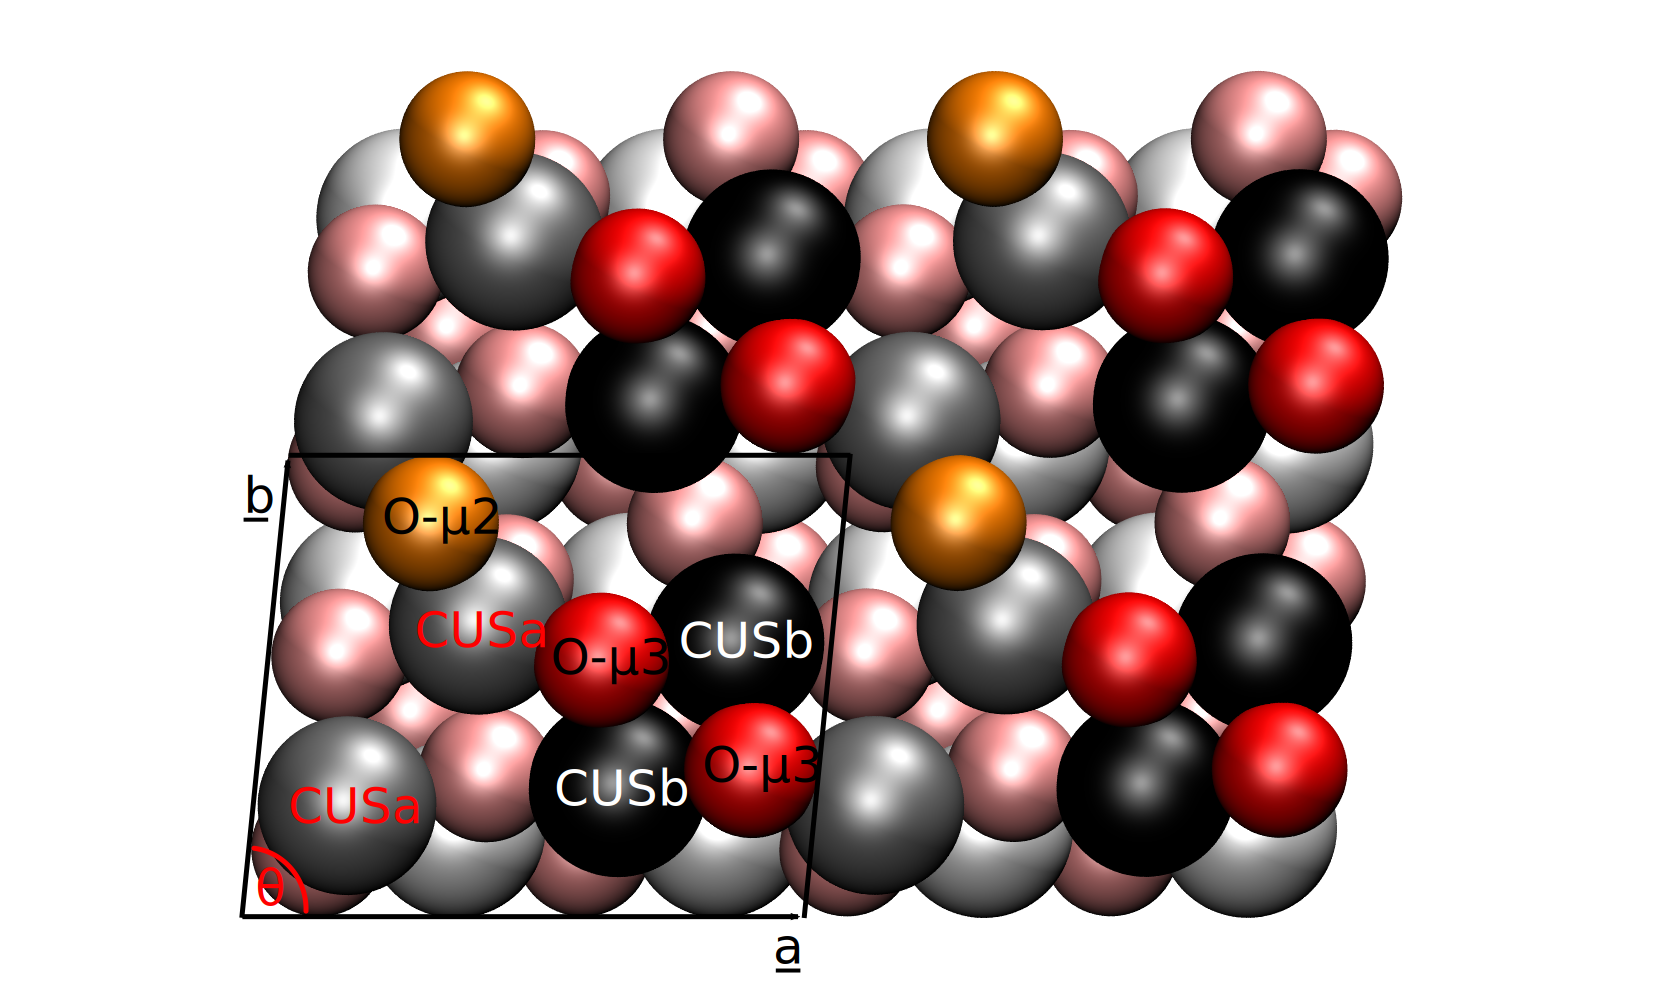
\includegraphics[width=0.4\textwidth]{figures/structures/supercell_opt.png}}%Abbildungen/new-surface-pictures/surface_top.png}}%
         \qquad
         %add desired spacing between images, e. g. ~, \quad, \qquad, \hfill etc. (or a blank line to force the subfigure onto a new line)
	 \subfigure[side view]{\includegraphics[width=0.4\textwidth]{figures/structures/uc_opt.png}}%Abbildungen/new-surface-pictures/surface-side.png}}%surf-seite-label.png}}
\caption{The (2$\times$2) $\alpha$-Al$_2$O$_3$(11\=20) surface model used in this work. (a) Top view, with the (1$\times$1) unit cell enclosed by the $\vec{a}$ and $\vec{b}$ lateral lattice vectors. Also shown are the two types of unsaturated  Al ions (CUSa (darker grey) and CUSb (black)), and two-  and threefold surface oxygen atoms (O-$\mu_2$ (orange) and O-$\mu_3$ (red)). Bulk atoms are in pale colours (Al light grey and O pale red). (b) Side view (only front-side of the unit cell), indicating two five-layer, \textit{i.e.}\ O-O$_2$-Al$_4$-O$_2$-O$\cdots$, sequences. The upper five-layers (above the solid line) were always relaxed, the lower five-layers (below the solid line) kept fixed at the bulk geometry.}
       \label{abb:unitcell}
\end{figure}
%
The atomic layer sequence of the (1$\times$1) $\alpha$-Al$_{2}$O$_{3}$(11\=20) surface is O-O$_2$-Al$_4$-O$_2$-O (where the indices give the number of atoms per layer in the (1$\times$1) unit cell) and that of a (2$\times$2) consequently O$_4$-O$_8$-Al$_{16}$-O$_8$-O$_4$. Two of these sequences, \textit{i.e.} ten atomic layers with 48 O and 32 Al atoms in total, were used in the calculations.
%{\color{blue} \sout{In Figure \ref{abb:unitcell}(b), three five-layer sequences are shown of which the  lowest one (below the dashed line) was cut off and not considered in our calculations.}}
The upper five-layers (above the solid line in Figure \ref{abb:unitcell}(b)) were optimised to allow for surface relaxation while the lower five-layers were fixed at the bulk geometry. Test calculations including more layers are shown in the Supporting Information, confirming that our choice is sufficiently accurate even for vibrational frequencies and 
 reaction pathways. 

The (1$\times$1) unit cell enclosed by a parallelogram with lattice vectors $\vec{a}$ and $\vec{b}$ of Figure~\ref{abb:unitcell}(a), has a topmost layer of oxygen (called the O layer) in which each O atom is coordinated to two Al atoms of the underlying lattice. Below this layer is a second oxygen layer (called the O$_2$ layer in the (1$\times$1) nomenclature of Figure~\ref{abb:unitcell}(b)). Oxygen atoms in the O$_2$ layer are three-fold coordinated by Al atoms. Following the usual nomenclature in coordination chemistry, we here denote these two types of O atoms O-$\mu_2$ and O-$\mu_3$ \cite{iupac-bridge}. Note that, in previous studies, they have also been described as Al$_{2}$O and Al$_{3}$O\cite{sung2012107}. Below these surface oxygens are a layer of surface Al atoms (called Al$_4$ in Figure \ref{abb:unitcell}(b)). Within this layer there are two different coordinatively unsaturated (CUS) Al atoms, called here CUSa and CUSb \cite{catalano2006108}. As is hopefully clear from inspection of Figure \ref{abb:unitcell}, CUSa Al atoms are covalently bound to one O-$\mu_2$, one O-$\mu_3$ and three deeper lying oxygens, while CUSb Al atoms are covalently bound to two O-$\mu_3$ and three deeper lying oxygens.    

Altogether, in the upper three layers of the O$_4$-O$_8$-Al$_{16}$ (2$\times$2) cell, we have 16 CUS Al sites, four O-$\mu_2$, and eight O-$\mu_3$ sites. The lateral cell vectors (for (1$\times$1)) are $|\vec{a}|=7.08\,$\AA{} and $|\vec{b}|=5.18\,$\AA{} and are fixed to their bulk values. The angle between the two lateral vectors is $84.56^{\circ}$. Adopting a supercell model, we repeat the ten-layer slab perpendicular to the surface with wide vacuum regions between individual ten-layer slabs. The ``$\vec{c}$-vector'' was chosen perpendicular to the surface with a length of $20.5\,$\AA. The resulting vacuum gap ($\sim 17\,$\AA) was large enough to avoid spurious interactions between individual ten-layer slabs. Using this supercell model and optimising the coordinates of the upper five-layer sequence (\textit{i.e.}\ below the solid line \textbf{(should be above?)} in Figure \ref{abb:unitcell}(b)) while fixing the rest to, theoretical, bulk values, to mimic the situation in the solid, the relaxed distances between the first five atomic layers are (bulk values are given in brackets for comparison) for the naked surface, in \AA: $d_{12}=0.232$ (0.193) (O-O$_2$ layer distance), $d_{23}=0.642$ (0.741) (O$_2$-Al$_4$), $d_{34}=0.656$ (0.741) (Al$_4$-O$_2$), and $d_{45}=0.198$ (0.191) (O$_2$-O), see also Figure \ref{abb:unitcell}(b). That is, the distance between the upper two oxygen layers ($d_{12}$) increases by about 20$\%$, and that of the second oxygen layer and the underlying Al layer ($d_{23}$) shrinks by about 13$\%$. The size of these relaxations are in near quantitative agreement with a prior study by Kurita and coworkers\cite{kuri10} who employed a different gradient-corrected density functional approach.

After optimising the UHV surface termination, a single water molecule per (2$\times$2) cell was then brought onto the surface, corresponding to a low coverage situation as in experiment (see below). In the computational model, the coverage is 1/16 when referring to the number of vacuum-exposed CUSa and CUSb sites (or 1/12 if considering CUSb and ``inter-CUSa'' (see below for definition) sites). Stable structures with adsorbed water and water fragments were found by optimising water and, again, the topmost five-layer slab.

For evaluating thermodynamic properties, Gibbs free energies $G(T)$ were determined for stable species and transition states, according to
\begin{equation}
 G(T) = H(T) - T \ S(T) \approx E + G^\mathrm{vib}(T)
\end{equation}
with the enthalpy $H(T)$, the entropy $S(T)$, the absolute temperature $T$, the self-consistent field (SCF) total energy $E$ and the vibrational part of the free energy, $ G^\mathrm{vib}(T)$. As we and others have discussed previously \cite{kirsch2014}, other contributions to $G$, \textit{e.g.}\ translation and rotation, cancel at surfaces. The vibrations were determined in the harmonic approximation by diagonalising the dynamical matrix at the $\Gamma$-point. Only coordinates arising from atoms that were not frozen were considered.
%  No scaling of frequencies was adopted.
The resulting frequencies are reported without scaling factors. Frequency analysis was done for H$_2$O and fragments if thermodynamic properties and rates were of interest, and for D$_2$O and its fragments if vibrational spectra were to be interpreted.

Because understanding the reactivity of water on the (11\=20) surface requires understanding the rates of inter-conversion of the various possible forms of interfacial water, we calculated canonical reaction rates for the reactions describing such inter-conversions using Eyring's transition state theory, 
\begin{equation} 
 k(T)=\frac{k_BT}{h}e^{-\Delta G^{\ddagger}(T)/k_BT} .
 %\kappa \ \frac{k_BT}{h}e^{-\Delta G^{\ddagger}(T)/k_BT}= \kappa \ k_0 \quad .
\label{eyr}
\end{equation}
Here, $h$ and $k_B$ are Planck's and Boltzmann's constants, and $\Delta G^\ddagger=G^\ddagger-G(\mbox{educt})$ is the activation free energy for the reaction in question, with $G^\ddagger$ being the free energy of the transition state. We located the transition state using the Nudged Elastic Band (NEB) with Climbing Image (CI) method~\cite{Henkelman00b,climbing-image}. We confirmed that each state resulting from these analyses was, in fact, a transition state by performing a frequency calculation and finding a single imaginary frequency. In contrast all minimum energy structures have only real frequencies.
%%%%%%%%%%%%%%%%%%%%%%%%%%%%%%%%%%%%%%%%%%%%%%%%%%%%%%%%%%%%%%%%%%%%%%%%%%%%%%%%%%%%%%%%%%%%%%%%%%%%%%%%%%%%%%%%%%%%%%%%%%%%%%%

\subsection{Experiment}\label{ss:exp}
All of the measurements described here were performed in a UHV chamber with a base pressure of $ 2.5 \times 10^{-10}$ mbar. All samples used in this study are $\alpha$-Al$_{2}$O$_{3}$(11\=20) single crystals, $10\times15\times0.5\,$mm$^3$, with one side polished to a roughness <0.5 nm, purchased from Princeton Scientific Co. Before installation into our chamber the received sample was sonicated in ethanol and in Mili-Q water, each for 15 min. After drying in N$_{2}$ we then mounted it in our chamber (the sample mounting was the same as that employed previously by us and others \cite{Elam96,kirsch2014,wirth2016characterization}). After sample mounting and bake out of the chamber, the sample surface was sputtered with Argon at $1000\,$keV for 30 min at multiple points and a pressure of  $1.0 \times 10^{-5}\,$mbar, annealed to $1200\,$K under UHV conditions and then annealed in oxygen at temperatures up to $1200\,$K for 10 min. After preparation the sample was confirmed to be carbon free using Auger spectroscopy and its surface structure checked by low energy electron diffraction (see Supporting Information for sample preparation details and results from these control experiments).  

After sample preparation water molecules (D$_2$O) were introduced into the chamber using a turbo molecular beam source (MBS) described in depth in previous work \cite{ceye88,mcca00}. In preliminary experiments we determined empirically that employing this MBS dramatically enhanced water adsorption relative to introduction into the chamber employing a leak valve. In parallel to the optical spectroscopy, described below, we also conducted Temperature Programmed Desorption (TPD) measurements to estimate water surface coverage using a quadrupole mass spectrometer (Satellite LM61) attached to our UHV chamber. The details of these measurements are further discussed both below and in the Supporting Information.

We characterize the vibrational response of interfacial OD stretch oscillators using vibrational sum frequency (VSF) spectroscopy. To conduct a VSF measurement the output of pulsed 800 nm (VIS) and mid-infrared (IR) lasers are overlapped spatially and temporally at an interface and the emission at the sum of the frequencies of the incident fields monitored. Our light source for these measurements is a Legend Elite Duo amplifier system (Coherent) with an output power of $8\,$mJ at $800\,$nm, 1 kHz repetition rate and $\approx50\,$fs pulse duration. $5\,$mJ of this pulse energy is sent to a TOPAS and difference frequency generation unit (Coherent) to generate IR pulses centered at $2780\,$cm$^{\text{-1}}$ with a FWHM of $190$-$240\,$cm$^{\text{-1}}$. The residual of the signal/idler generation in the TOPAS is narrowed using a free space etalon to produce pulses centered 800 nm with a spectral bandwidth of $8\,$cm$^{\text{-1}}$. After traversing through a series of mirrors, $\frac{\lambda}{2}$ plate/polarizer combinations, and lenses the IR and narrowed 800 nm beams are brought to the sample with incident angles of 70$^\circ$ and 75$^\circ$ respectively (both beams copropagate in a plane normal to the sample surface, angles are defined with respect to the surface normal).  The emitted field at the sum of the frequencies of the two incident beams is collimated, propagated to a spectrograph (Triax 320, Horiba Scientific) and dispersed onto an emCCD camera (Andor Scientific) for detection. All data was collected in the (SF/VIS/IR) \textit{ppp} polarization condition (where \textit{p} indicates parallel to the incident plane). All samples from which VSF spectra were collected were held at 130 K during measurement. Control experiments suggest that, at this temperature, the spectral response is stable over > 2 days. Because our infrared source (described below) is more intense at OD than OH stretch frequencies, all experimental results reported below employed \ce{D2O} instead of \ce{H2O}.

As extensively reviewed in the literature the emitted sum frequency field is interface specific by its symmetry selection rules (in the dipole approximation) and is a spectroscopy because, at frequencies at which the incident IR field is in resonance with an interfacial vibration a several order of magnitude increase in emitted intensity can be observed \cite{lam05}. To quantify this VSF spectral response we followed prior workers and modelled the signal as the coherent sum of a nonresonant and, possibly, multiple resonant, contributions  \cite{bain91}. 

If each resonance is homogeneously broadened and dynamical effects can be neglected (see the Supporting Information of our prior work describing \ce{D2O} adsorption on $\alpha$-\ce{Al2O3}(0001) for a detailed justification of this point \cite{kirsch2014}), $\text{I}_\text{vsf}$ can be described as,
\begin{equation}\label{e:line1}
\text{I}_{\text{vsf}} \propto \left| \chi_\text{eff}^{(2)} \right|^2 \text{I}_{\text{vis}}\text{I}_{\text{ir}}(\tilde{\nu}_{\text{ir}}) \quad
\end{equation}
%
where $\text{I}_{\text{vis}}$ is the intensity of the visible beam, $\text{I}_{\text{ir}}(\tilde{\nu}_{\text{ir}})$ is the, frequency dependent, intensity of the infrared pulse and $\chi^{(2)}_\mathrm{eff}$ is the effective second order macroscopic susceptibility, given as 
\begin{eqnarray}
\chi_{\text{eff}}^{(2)} & \propto & \chi^{(2)}_{\text{nr}} + \chi^{(2)}_{\text{r}}\nonumber\\  
	& \propto & \left|\text{A}_{\text{nr}}\right|e^{i\phi_\text{nr}} + \sum_{q} \frac{\text{A}_{q}}{\tilde{\nu}_{\text{ir}}-\tilde{\nu}_q + i\Gamma_q}e^{i\phi_{q}}\label{e:line2}
\end{eqnarray}
where $\chi^{(2)}_{\text{r}}$ is the resonant and $\chi^{(2)}_{\text{nr}}$ the nonresonant portion of $\chi^{(2)}_{\text{eff}}$, $\text{A}_{\text{nr}}$ the amplitude of the nonresonant contribution, $\phi_{\text{nr}}$ the phase of the nonresonant contribution, $\tilde{\nu}_{\text{ir}}$ the infrared frequency, and $\text{A}_{q}$ the amplitude, $\phi_{q}$ the phase, $\tilde{\nu}_{q}$ the center frequency, and $2\Gamma_q$ the line width of resonance \textit{q}. As reviewed in detail in a variety of previous references and in the Supporting Information, $\text{A}_{q}$ is proportional to the number of molecules in the laser focus (\textit{i.e.}\ or, equivalently, I$_{\text{vsf}}$ is proportional to the number of molecules squared) and their ensemble averaged orientation. As discussed below and in detail in the Supporting Information, the theoretical description of this relationship is well developed in the literature and makes it possible, given incident beam angles and polarizations, to calculate the expected measured I$_{\text{vsf}}$ as a function of molecule orientation\cite{zhu99,lam05}.  



%%%%%%%%%%%%%%%%%%%%%%%%%%%%%%%%%%%%%%%%%%%%%%%%%%%%%%%%%%%%%%%%%%%%%%%%%%%%%%%%%%%%%%%%%%%%%%%%%%%%%%%%%%%%%%%%%%%%%%%%%%%%%%%


\section{Results and Discussion}
\subsection{Computation and Theory\label{sec3}}

\subsubsection{Molecular and dissociative adsorption}
Given the $\alpha$-\ce{Al2O3} surface model and computational approach described above we find one molecularly, and several dissociatively adsorbed configurations for a single water molecule in one ($2\times 2$) supercell. These minimized structures are shown in Figure \ref{abb:ads-geoms} and their adsorption energies and free energies tabulated in Table \ref{tab_energies}. As we discuss further below, other structures, \textit{e.g.}\ those with greater separation of the OH (or OH$^-$) and H (or H$^+$) fragments of the adsorbed \ce{H2O} are all higher in energy.  

\begin{figure}[!h]
 \centering
\subfigure[CUSb]{\includegraphics[width=0.2\textwidth]{figures/structures/test-Cb.pdf}}
 \quad\quad
 \subfigure[inter-CUSa||O-$\mu_2$]{\includegraphics[width=0.2\textwidth]{figures/structures/test-iCa2.pdf}}
  \quad
\subfigure[CUSb||O-$\mu_2$]{\includegraphics[width=0.2\textwidth]{figures/structures/test-Cb2.pdf}}
 \quad
\subfigure[inter-CUSb||O-$\mu_2$]{\includegraphics[width=0.2\textwidth]{figures/structures/test-iCb2.pdf}}
\quad
\subfigure[inter-CUSa||O-$\mu_3$]{\includegraphics[width=0.2\textwidth]{figures/structures/test-iCa3.pdf}}
 \quad
\subfigure[CUSb||O-$\mu_3$]{\includegraphics[width=0.2\textwidth]{figures/structures/test-Cb3.pdf}}
 \quad
\subfigure[inter-CUSb||O-$\mu_3$]{\includegraphics[width=0.2\textwidth]{figures/structures/test-iCb3.pdf}}
 \caption{Adsorption geometries for molecular (a) and (six) dissociated water molecules ((b)-(g)) are shown, as obtained by periodic PBE+D2. The most favorable molecularly and dissociatively adsorbed configurations are shown. This means that we show nearest neighbour structures only (see text). The colour code is the same as in Figure \ref{abb:unitcell}, CUSa grey, CUSb black, O-$\mu_2$ orange and O-$\mu_3$ red; Hydrogen is displayed in white, subsurface layers are in pale colours.}
        \label{abb:ads-geoms}
 \end{figure}

%%%%

\begin{table*}[!h]
  \centering
 \caption{Adsorption energies $E_\textrm{ads}=E_\text{ads. species}-E_\text{free molecule+surface}$ for molecular and (singly) dissociated water on $\alpha$-\ce{Al2O3}(11\=20) according to periodic PBE+D2 calculations. The corresponding adsorption free energies $G_\textrm{ads}$ at 130, 300 and 400 K defined analogously are also given. Three most stable configurations are in bold. All energies are in eV. 
\vspace*{.2cm} 
  }
  \begin{tabular}{cl|cccc}
   \multicolumn{2}{c|}{Adsorbed Species}  & $E_\text{ads}$ & $G_\text{ads, 130 K}$  &  $G_\text{ads, 300 K}$  & $G_\text{ads, 400 K}$ \\
\hline
\multirow{1}{*}{molecular} & CUSb          &   -1.78  &-1.60 & -1.51  & -1.46 \\
  \hline
 \multirow{6}{*}{dissociated} & \bf inter-CUSa||O-$\mu_2$ & \bf-2.50 &-2.27 & -2.16 & -2.09 \\
  & inter-CUSa||O-$\mu_3$ & -1.67 &-1.44 &-1.33 & -1.27 \\
  & \bf CUSb||O-$\mu_2$ & \bf -2.28 & -2.12& -2.03 &-1.97  \\
 & CUSb||O-$\mu_3$ & -1.19 &-1.05 &-0.98 & -0.95 \\%Cb3_other
 & \bf inter-CUSb||O-$\mu_2$ & \bf -2.09 &-1.88 &-1.80 & -1.76 \\
 & inter-CUSb||O-$\mu_3$ & -1.89 &-1.71 & -1.63 & -1.58 \\
  \end{tabular}
  \label{tab_energies}
\end{table*}
%%%%%


As is shown in Figure \ref{abb:ads-geoms} and Table \ref{tab_energies} molecularly adsorbed water tends to interact with the (11\={2}0) surface through its oxygen: surface unsaturated Al$^{+3}$ cations act as Lewis acids. As described above, the (11\=20) surface has two types of coordinatively undersaturated surface Al$^{+3}$ atoms: CUSa and CUSb sites. Our structure search suggests that a single water molecule will adsorb on a CUSb site, with an adsorption energy of -$1.78\,$eV. 
 Molecular adsorption above or between two adjacent CUSa sites (``inter-CUSa'' in what follows) 
 or between two adjacent CUSb sites (``inter-CUSb'') does not take place at the 
 level of theory employed in this study:
 geometry optimizations starting from molecular water placed above either of \textbf{(is ``either of'' correct?)} these sites at different heights converge to 
% a tendency of forming a stable inter-CUSa molecular species, however, they always lead to 
 dissociative species. It cannot be excluded with complete certainty, however, 
 that  molecular adsorption sites other than CUSb could be found when applying different 
 starting structures and / or 
 electronic structure methods.

Water dissociative adsorption is facilitated by the fact that the Lewis acid character of CUSa and CUSb surface aluminium atoms also allows them to act as adsorption sites for \ce{OH-} groups following the dissociative adsorption of \ce{H2O}. As shown in Figure \ref{abb:ads-geoms} and Table \ref{tab_energies}, in practice we find that this OH fragment adsorbs only in the CUSb, inter-CUSb or inter-CUSa positions. In principle the other fragment of a dissociatively adsorbed water molecule, \textit{i.e.}\ the H$^{+}$, can adsorb at either of the two possible surface Lewis base sites: the O-$\mu_2$ or the O-$\mu_3$. In practice we find that all six possible next neighbour combinations of \ce{OH-} and \ce{H+} adsorption sites are minima in our model chemistry (see Table \ref{tab_energies}). In what follows we employ the terminology \textsf{OH$^{-}$ site}||\textsf{H$^{+}$ site} (\textit{e.g.}\ CUSb||O-$\mu_2$) to characterize the dissociatively adsorbed complex. Configurations where the \ce{OH-} and \ce{H+} fragments from water are not at their nearest neighbour sites, perhaps due to OH or H diffusion, are denoted with O-$\mu_x^\prime$.

For the six dissociated minima we find adsorption energies $E_\text{ads}$ between -$1.19\,$eV for the CUSb||O-$\mu_3$, and -$2.50\,$eV for inter-CUSa||O-$\mu_2$ configurations (see Table \ref{tab_energies}). In general, we find that configurations in which the \ce{H+} fragment adsorbs on O-$\mu_2$ sites are more favourable than those in which it adsorbs on O-$\mu_3$. We rationalise this trend by noting the lower negative charge and smaller basicity of O bound to three Al atoms. The three most stable dissociatively adsorbed configurations, inter-CUSa||O-$\mu_2$, CUSb||O-$\mu_2$ and inter-CUSb||O-$\mu_2$, have energies clearly lower than the molecularly adsorbed species. As a consequence, dissociation starting from either molecular adsorbate is exoenergetic, by up to -$2.28\,$eV-(-$1.78\,$eV) = -$0.5\,$eV (for the formation of CUSb||O-$\mu_2$). While the thermodynamic picture thus seems clear, to fully characterize surface structure it is desirable to understand the kinetics of interconversion between minimum energy structures 
of each of the adsorbed species.
 
  
\subsubsection{Reaction Kinetics}
To do so we next employed Eyring transition state theory in combination with Nudged Elastic Band (NEB) transition state/minimum energy path search as outlined above. 
%Given the minimum energy adsorbate configurations, there are basically {\color{blue}two possible relevant dissociation reactions.

We first consider a molecular dissociation reaction (D-I) which connects 
 the molecular adsorbed state, H$_2$O(CUSb), with the second most 
 stable dissociated state of Table \ref{tab_energies},  CUSb||O-$\mu_2$,
%
\begin{equation}
 \mbox{H$_2$O (CUSb)}  \rightarrow  \mbox{OH(CUSb) + H (O-$\mu_2$)} \tag{D-I}
\label{diss1}
\end{equation}
%
where a favoured O-$\mu_2$ oxygen is protonated. As shown in Table \ref{tab:reaction-rates} and Figure \ref{mep}(a), this reaction is exoenergetic and exergonic: $\Delta E = E(\text{product})-E(\text{educt})= -0.50\,$eV, and $\Delta G_{\text{300 K}}= G(\text{product})-G(\text{educt})=-0.52\,$eV. Using 
 NEB analysis and PBE+D2 we find only 
 a very small energetic barrier for this reaction, $\Delta E^\ddagger=0.01\,$eV, 
  and an even smaller free energy barrier $\Delta G^\ddagger_{300K}=0.002\,$eV, leading 
 formally to a classical  
 dissociation rate constant at $300\,$K of $k_{300K}=5.76\times 10^{12}\,$s$^{-1}$, {\it cf.} Table \ref{tab:reaction-rates}.
 We expect this (and indeed all barriers) to be underestimated at the GGA level of theory \cite{Zhao05}.
 Still, comparing 
 the calculated  barriers to analogous dissociation reactions on (0001) and (1\=102) surfaces 
 applying the same method,
 suggests that (11\=20) is the most reactive of the three surfaces \cite{Wirth12,wirth2016characterization} with respect to 
dissociation: as will be discussed in more detail below (Table 
 \ref{comparison_surf}) the fastest dissociation reactions on (0001) and (1\=102) have 
 GGA activation free energies at 300 K above 0.1 eV and 
 corresponding rate constants of $8\times10^{10}$ and $5.2\times10^{10}\text{ s}^{-1}$, respectively.

A second possible molecular dissociation reaction (D-II) is,
%
\begin{equation}
 \mbox{H$_2$O (CUSb)}  \rightarrow  \mbox{OH(CUSb) + H (O-$\mu_3$)} \tag{D-II}
\label{diss2}
\end{equation}
%
leading to a less favourable O-$\mu_3$ protonation from the molecular CUSb state: CUSb||O-$\mu_3$. Indeed 
this reaction is endoenergetic ($\Delta E=0.59\,$eV) and endergonic ($\Delta G=0.53\,$eV), with 
 a NEB reaction path as shown in Figure \ref{mep}(b). For this reaction no additional 
 energy barrier $\Delta E^\ddagger=E^\ddagger-E(\mbox{products})$ could be found with the present numerical settings of the NEB calculations, despite both educt and product being minima. No rate was calculated in this case but the reaction will 
 be comparatively 
 slow since the activation free energy is at least as large as $\Delta G=0.53\,$eV.

{\color{red}Other dissociated minima as listed in 
 Table \ref{tab_energies} cannot be easily reached directly from 
 the molecularly adsorbed CUSb species, at least not in a single 
 step, since both the OH and H fragments will have to move after 
 dissociation.} 
 {\color{green}[Is being checked at the moment by Sophia.]} 
Due to the high reactivity 
 of H$_2$O(CUSb) w.r.t. dissociation 
 into the CUSb||O-$\mu_2$ state, it is expected 
 that this reaction channel dominates initially.
 Once the CUSb||O-$\mu_2$ has been formed, however,
 the other stable dissociated species, 
 inter-CUSb||O-$\mu_2$ and inter-CUSa||O-$\mu_2$, can 
 be reached.
 For instance,
 the rotation of the water-hydroxyl fragment in CUSb||O-$\mu_2$ around the CUSb site into an inter-CUSb position leaving the proton at its original O-$\mu_2$ position can be considered as a 
 diffusion reaction (Df) of OH, leading to inter-CUSb||O-$\mu_2$, the third most 
 stable species according to Table \ref{tab_energies}:
 \begin{equation}
 \text{OH(CUSb)} + \text{H(O-$\mu_2$)}
  \rightarrow \text{OH(inter-CUSb)} + \text{H(O-$\mu_2$)} \tag{Df-OH-III}
  \label{diffOH3}
\end{equation}
The calculated reaction path is shown in Figure \ref{mep}(c). 
 The process is slightly endoenergetic/endergonic (by \textasciitilde$0.2\,$eV), and has a barrier of 
 $\Delta E^\ddagger=0.35\,$eV/$\Delta G^\ddagger_{300K}=0.39\,$eV. The corresponding $k_{300K}$ is $\approx 1.8\times 10^6\,$s$^{-1}$ (see Table \ref{tab:reaction-rates}).

In another OH ``diffusion'' reaction the 
  OH fragment of CUSb||O-$\mu_2$ moves from a CUSb-position to inter-CUSa with the proton staying at its initial, next-neighbour, 
 O-$\mu_2$ position,
  leading to the most stable  inter-CUSb||O-$\mu_2$ dissociated 
 state (Figure \ref{mep}(d)):
 \begin{equation}
 \text{OH(CUSb)} + \text{H(O-$\mu_2$)}
  \rightarrow \text{OH(inter-CUSa)} + \text{H(O-$\mu_2$)} \tag{Df-OH-IV}
    \label{diffOH4}
\end{equation}
This process is exoenergetic/exergonic since the inter-CUSa||O-$\mu_2$ is $0.22$\,eV more stable than the CUSb||O-$\mu_2$. 
With a barrier of $\Delta E^\ddagger=1.07\,$eV/$\Delta G^\ddagger_{300K}=1.10\,$eV, however, 
  this reaction appears to be 
 slow (at least when compared to Df-OH-III) with a rate at $300\,$K of $k_{300K}=2.41\times 10^{-6}\,$s$^{-1}$. 
 Our prior work on both the (0001) and (1\=102) surfaces shows that this process of CUS to CUS OH-diffusion is essentially 
 not possible on these surfaces \cite{kirsch2014,wirth2016characterization}, due to even  higher 
 activation energies.
% but since this reaction is not directly from CUSb to CUSb but to an inter-CUSa position that is not that far away and sterically hindered as the diffusion to another CUSa´b, this might be an exception.

In addition to diffusion of OH fragments one might also imagine the diffusion of adsorbed H$^+$ (or H). We investigated two of the possible diffusion reactions of this type (see Figure \ref{mep2}). The first is a H 
 diffusion from O-$\mu_2$ to  O-$\mu_3$ with the OH adsorbed on an inter-CUSa site:
 \begin{equation}
 \text{OH(inter-CUSa)} + \text{H(O-$\mu_2$)}
  \rightarrow \text{OH(inter-CUSa)} + \text{H(O-$\mu_3^\prime$)} \tag{Df-H-V}
     \label{diffH5}
\end{equation}
Here the prime indicates that we consider the second-nearest neighbour O-$\mu_3$ site, rather than a nearest neighbour O-$\mu_3$.
 The corresponding minimum energy path from a NEB calculation
 is shown in Figure \ref{mep2}(a).
 From there (as shown in 
Table \ref{tab:reaction-rates}) 
 we  see that the reaction is significantly endoenergetic/endergonic, 
%with $\Delta E^\ddagger=01.65\,$eV/$\Delta G^\ddagger_{300K}=1.49\,$eV and a reaction rate constant of $k_{300K}=4.90\times 10^{-13}\,$s$^{-1}$
 due to the energetically costly protonation of an O-$\mu_3$ site, plus the additional energy needed to move the proton farther from the  stabilizing OH ion. The corresponding activation free energy at 300 K is $\approx 1.49\,$eV and the corresponding classical rate constant therefore very small, $k_{300K}=4.90\times 10^{-13}\,$s$^{-1}$.
 {\color{red}In general, diffusion reactions
 with H traveling from O-$\mu_2$ to O-$\mu_3$ sites are energetically 
 costly and often show additional barriers, making 
 these processes probably unmeasurably slow.} 
%This rather slow reaction can be understood since the very stable O-$\mu_2$-adsorbed H diffuses to a less stable O-$\mu_3$ position and also the distance between the OH and H fragments is larger so that there is less stabilization.

The second type of H-diffusion reaction we studied is
 \begin{equation}
 \text{OH(inter-CUSb)} + \text{H(O-$\mu_3^{\prime\prime}$)}
  \rightarrow \text{OH(inter-CUSb)} + \text{H(O-$\mu_3^{\prime\prime\prime}$)} \tag{Df-H-VI}
     \label{diffH6}
\end{equation}
where  H diffuses from an O-$\mu_3$ site to another, neighbouring 
  O-$\mu_3$ position (Figure \ref{mep2}(b)). Double and triple primes 
 indicate third- and fourth-nearest neighbours in this 
 case. The adsorption energies for educts and products are similar now
 ($\Delta E=-0.06\,$eV/$\Delta G=-0.07\,$eV) because the only difference is the distance between OH and H fragments. 
 Still, the barrier is quite high with $\Delta E^\ddagger=1.05\,$eV and $\Delta G^\ddagger_{300K}=0.94\,$eV, resulting 
  in a rate constant of $k_{300K}=1.05\times 10^{-3}\,$s$^{-1}$. 


\begin{figure*} [!h]
\centering
\subfigure[D-I: CUSb $\rightarrow$CUSb||O-$\mu_2$]{\includegraphics[width=0.7\textwidth]{figures/structures/mep_paths/Diss_Cb-Cb2.pdf}}
         \quad
\subfigure[D-II: CUSb $\rightarrow$CUSb||O-$\mu_3$]{\includegraphics[width=.7\textwidth]{figures/structures/mep_paths/Diss_Cb-Cb3.pdf}}
 \quad
\subfigure[Df-OH-III: CUSb||O-$\mu_2$ $\rightarrow$inter-CUSb||O-$\mu_2$]{\includegraphics[width=.7\textwidth]{figures/structures/mep_paths/Diff-OH_Cb2-iCb2.pdf}}
 \quad
\subfigure[Df-OH-IV: CUSb||O-$\mu_2$ $\rightarrow$inter-CUSa||O-$\mu_2$]{\includegraphics[width=.7\textwidth]{figures/structures/mep_paths/Diff-OH_Cb2-iCa2.pdf}}
\caption{Minimum energy paths with transition states (inlay; if available), 
  and both educt (left) and product (right) states for D-I, D-II, Df-OH-III and Df-OH-IV reactions, respectively. The colour code is as explained above.}
       \label{mep}
\end{figure*}
\begin{figure*} [!h]
\centering
\subfigure[Df-H-V: inter-CUSa||O-$\mu_2\rightarrow$inter-CUSa||O-$\mu_3^\prime$]{\includegraphics[width=.7\textwidth]{figures/structures/mep_paths/Diff-H_iCa2-iCa3p.pdf}}
 \quad
\subfigure[Df-H-VI: inter-CUSb||O-$\mu_3^{\prime\prime}$ $\rightarrow$inter-CUSb||O-$\mu_3^{\prime\prime\prime}$]{\includegraphics[width=.7\textwidth]{figures/structures/mep_paths/Diff-H_iCb3pp-iCb3ppp.png}}
\caption{Minimum energy paths with transition states, 
  and both educt and product states for Df-H-V and Df-H-VI reactions, respectively. The colour code is as explained above.}
       \label{mep2}
\end{figure*}


\begin{table*}[ht]
  \centering
  \caption{Reaction rates for selected reaction paths examined. $\Delta E=E(\textrm{product}) - E(\textrm{educt})$, $\Delta E^{\ddagger}=E^\ddagger - E(\textrm{educt})$,
  respectively for the free energy, $G$.  
 $k$ is the rate constant from eq.~(\ref{eyr}). Thermodynamic quantities and rates are given
  for $T=300\,$K. ``n.f.'' indicates ``not found''.
Reactions 
 I-VI are are defined in the text and are either 
 water dissociations (D), OH diffusion (Df-OH) 
 or H diffusions (Df-H). 
  }
  \begin{tabular}{cl|cc|cc|c}
  \multicolumn{2}{c|}{Reaction Type}             & $\Delta E$ (eV)& $\Delta G_\text{300 K}$ (eV) &$\Delta E^{\ddagger}$ (eV) & $\Delta G_\text{300 K}^{\ddagger}$ (eV) & $k_\text{300 K}$ (s$^{-1}$)  \\%& $\kappa$\\
    \hline 
\multirow{2}{*}{\ce{H2O} dissociation} &
   D-I  & -0.50 & -0.52 & 0.01 & 0.002 & 5.76$\cdot 10^{12}$ \\
 & D-II & 0.59 &0.53 & n.f. & n. f. & n. f. \\
    \hline
 \multirow{2}{*}{OH diffusion} &
   Df-OH-III & 0.19 & 0.22 & 0.35 & 0.39 & 1.8$\cdot 10^6$\\
 & Df-OH-IV  & -0.21 & -0.13 & 1.07 & 1.10 & 2.41$\cdot 10^{-6}$ \\
    \hline
\multirow{2}{*}{H diffusion} &
  Df-H-V  & 1.08 & 1.04 & 1.65 & 1.49 & 4.90$\cdot 10^{-13}$ \\
& Df-H-VI & -0.06 & -0.07 & 1.05 & 0.94 & 1.05$\cdot 10^{-3}$ \\
  \end{tabular}
  \label{tab:reaction-rates}
\end{table*}


In summary, while we cannot present a complete 
 kinetic network with all possible 
 reactions at the moment, already from the results above the following conclusions can be drawn:
 Starting from adsorbed, intact water, 
 dissociated species are readily formed: notably 
 CUSb||O-$\mu_2$ is easily accessible from the molecular CUSb state. The other two low-energy dissociated species, 
 inter-CUSa||O-$\mu_2$  and inter-CUSb||O-$\mu_2$ could be 
 reached at room temperature from 
 CUSb||O-$\mu_2$, by fast (inter-CUSb||O-$\mu_2$) and slow (inter-CUSa||O-$\mu_2$) reactions, respectively. 
 Dissociated species involving protonated 
 O-$\mu_3$ sites are energetically disfavoured and 
 their formation (from protonated
 O-$\mu_2$ sites) typically also kinetically hindered. 
 We conclude that the low-energy 
 dissociated species with protonated 
 O-$\mu_2$ sites will form on the surface in the course of time. 




\subsubsection{Vibrational Frequencies}
As mentioned above, in addition to the theoretical description of the thermodynamics and kinetics of water reaction with the (11\=20) surface we also conducted \textbf{v}ibrationally resonant \textbf{s}um \textbf{f}requency (VSF) spectroscopy measurements to characterize O-D stretching vibrations of (dissociated) D$_2$O. The details of these results, and how they connect to the picture of water reactivity emerging above, are discussed below. To aid in this comparison we calculated harmonic frequencies for the three most probable dissociatively adsorbed (D$_2$O) configurations: the inter-CUSa||O-$\mu_2$, CUSb||O-$\mu_2$, and inter-CUSb||O-$\mu_2$, with adsorption energies of -$2.50$, -$2.28$ and -$2.09\,$eV respectively (see Table \ref{tab_energies}).  Because, as discussed above, measured VSF intensities also strongly depend on OD orientation with respect to the laboratory reference frame we have included the, calculated, angle of each OD fragment with respect to the surface normal. These results are shown in the left half of Table \ref{tab:frequencies}. For later reference, we also include Boltzmann weights $P_i = \text{exp}(-G_i/k_BT)$ of these three most stable dissociated configurations for various temperatures relevant for this work, relative to the value for the most stable inter-CUSa||O-$\mu_2$ configuration, in the right half of the table. As noted above, we calculated free energies, and therefore also these weights, for dissociated H$_2$O rather than D$_2$O -- differences for D$_2$O are minor.
%
\begin{table*}[hbt]
  \centering
  \caption{Left half: Selected frequencies for the most stable structures of the three low-energy dissociated species, for OD stretching vibrations. $\theta$ is the angle between the O-D axis for adsorbed (``ads'') and surface (``surf'') hydroxyl and the surface normal. Right half: Boltzmann populations (relative to the value for the most stable configuration inter-CUSa||O-$\mu_2$) for the three low-energy dissociated species, at various temperatures.
}
%\vspace*{.2cm} \\
  \begin{tabular}{cl|cc|ccc}
   \multicolumn{2}{c|}{O-D type} & $\theta$ ($^{\circ}$) &  $\tilde{\nu}_{\textrm{OD}}$ (cm$^{-1}$) & $P_\text{130 K}$ & $P_\text{300 K}$ & $P_\text{400 K}$\\
    \hline
\multirow{2}{*}{inter-CUSa||O-$\mu_2$} & OD(inter-CUSa)   &44 & 2731 & \multirow{2}{*}{1} & \multirow{2}{*}{1} & \multirow{2}{*}{1}\\ % Al9-30_O56
 & D(O-$\mu_2$)   &36 & 2694 & & & \\
\hline
\multirow{2}{*}{CUSb||O-$\mu_2$} &  OD(CUSb) & 26 & 2785 & \multirow{2}{*}{$1.4 \times 10^{-6}$} & \multirow{2}{*}{$6.1 \times 10^{-3}$} & \multirow{2}{*}{$3.2 \times 10^{-2}$} \\ % Al26_34
& D(O-$\mu_2$) &60 &  1711 & & & \\
\hline
%\multicolumn{6}{|c|}{inter-CUSb||O-$\mu_2$}\\
 \multirow{2}{*}{inter-CUSb||O-$\mu_2$} & OD(inter-CUSb) &53 &  2692 & \multirow{2}{*}{$1.0 \times 10^{-15}$} & \multirow{2}{*}{$1.2 \times 10^{-6}$} & \multirow{2}{*}{$6.6 \times 10^{-5}$}\\ %Al3-10_O56
 & D(O-$\mu_2$)    &41 &  2689 & & & 
  \end{tabular}
\label{tab:frequencies}
\end{table*}

Inspection of these results suggests that in all cases the frequencies of OD groups originating in the adsorbed \ce{D2O} are larger than those of the OD formed by the adsorption of a deuteron on a surface O-$\mu_2$ or O-$\mu_3$. This trend can, in part, be explained by the slightly larger reduced mass of the D(O-$\mu_{2}$) oscillator. In the latter D is directly bound to an entire surface while in the former only to a quasi-free O \cite{kirsch2014}. However, as demonstrated in our prior studies, this effect is at largest tens of wavenumbers. Rationalizing, for example, the $1000\,$cm$^{-1}$ differences between the two OD oscillators in the CUSb||O-$\mu_2$ configuration likely requires an additional softening of the D(O-$\mu_{2}$) bond due to H-bonding.


\subsection{Experimental Results: Vibrations and their Assignment\label{res_exp}}
%
Our goal in this study is to develop a self-consistent experimental and theoretical view of water reactivity at low coverages on $\alpha$-\ce{Al2O3}(11\=20). As discussed above and in more detail in the Supporting Information, we created samples by dosing \ce{D2O} using our MBS while cooling to liquid nitrogen temperatures. This treatment leaves, a layer of dissociatively adsorbed \ce{D2O} overlain by an ice layer (presumably multilayers thick) on the $\alpha$-alumina surface. After being used for spectrometer alignment, the ice layer and some fraction of the dissociatively adsorbed water was removed by rapid annealing and the sample was returned to liquid nitrogen temperatures for collection of VSF spectra. \ce{D2O} surface coverage was quantified by collecting TPD spectra (Temperature Programmed Desorption) after VSF spectra were collected. These TPD measurements (see Supporting Information for the data) allow us to quantify that rapid annealing to 183 K produces a \ce{D2O} coverage of 1 ML, to $300\,$K a coverage of 0.14 ML and to $400\,$K a coverage of 0.05 ML:  in reasonable agreement with water coverages employed in calculation, (\textit{i.e.}\ 0.05-0.08 ML depending on the definition of adsorption {\it site}).
%
%\begin{widetext}
\begin{figure*}
\begin{center} 
\includegraphics[width=0.96\textwidth]{figures/spectra/SFG_data}
\end{center} 
\caption{VSF spectra of \ce{D2O} adsorbed on $\alpha$-\ce{Al2O3}(11\=20) at 0.14 ML surface coverage (left panel), after annealing to 300 K, and at 0.05 ML surface coverage (right panel), after annealing to 400 K.  The squared modulus of resonances resulting from the fit are plotted below each data set. Note that all VSF measurements are carried out when the sample is cooled to $130\,$ K after the indicated heating step.}
\label{G-SFG1}
\end{figure*}
%\end{widetext}

Figure \ref{G-SFG1} shows VSF spectra and fits to the data using the line shape model described above for samples with 0.14 ML coverage (\textit{i.e.}\ annealed to $300\,$K) and 0.05 ML coverage (\textit{i.e.}\ annealed to $400\,$K). As indicated, note that we divide the measured signal by its corresponding nonresonant response to account for the frequency dependence of our infrared source. Analyzing our data using the line shape model in equations \ref{e:line1} and \ref{e:line2} is an underconstrained minimization problem. To constrain this uncertainty we asked whether our data is well described making substantial simplifying assumptions: that there is the same number of resonances present at both surface coverages and their center frequency, line widths and phase are independent of coverage. Armed with these assumptions, and conducting a global fit of both data sets we find that applying the line shape model in equations \ref{e:line1} and \ref{e:line2}) gives a single strong and two weaker resonances centered at $2766\pm0.6$, $2814\pm5.5$ and $2843\pm 1.2\text{ cm}^{-1}$ respectively (see Supporting Information for further details of the data analysis).
%

To assign the three experimentally observed spectral features we first turn our attention to the calculated frequencies in Table \ref{tab:frequencies}. Clearly these frequencies cluster in four groups: the OD(CUSb) group from the CUSb||O-$\mu_2$ adsorbate configuration is highest at $2785\,$cm$^{\text{-1}}$, the OD(inter-CUSa) group from the inter-CUSa||O-$\mu_2$ configuration is somewhat lower at $2731\,$cm$^{\text{-1}}$, the D(O-$\mu_2$) group from the inter-CUSa||O-$\mu_2$, the OD(inter-CUSb) from the inter-CUSb||O-$\mu_2$ and the D(O-$\mu_2$) from the inter-CUSb||O-$\mu_2$ range from $2689$-$2694\,$cm$^{\text{-1}}$, and the D(O-$\mu_2$) from CUSb||O-$\mu_2$ is lowest frequency at $1711\,$cm$^{\text{-1}}$. It is not immediately obvious how the three resonances apparent in the experimental data relate to these four to six frequencies in calculation.

As mentioned above, the intensity of the measured emitted sum frequency field is proportional to the number of oscillators squared. To address the likely contribution of OD oscillators from each adsorbate configuration to our observed VSF spectra we need to know their relative populations. While kinetic trapping of unstable species cannot 
 be excluded with certainty,
%Because there is no evidence for the kinetic stabilization of particular adsorbate configurations 
we addressed this problem by assuming the surface was at thermal equilibrium and calculating Boltzmann probabilities of the inter-CUSa||O-$\mu_2$, CUSb||O-$\mu_2$ and inter-CUSb||O$\mu_2$ configurations. This analysis, for temperatures of $130$, $300$, and $400\,$K is shown in the right half of Table \ref{tab:frequencies}. Clearly, over the temperature range relevant in experiment we would expect to see only contribution from OD oscillators in the most stable inter-CUSa||O-$\mu_2$ or, perhaps, the second most stable CUSb||O-$\mu_2$ configurations.

While I$_{\text{vsf}}$ is proportional to oscillator population squared, it is also, as discussed above and in detail in the Supporting Information, a function of OD orientation. The details of the physics of this relationship, and the resulting equations, can be found in many prior studies and are reproduced in the Supporting Information here for reference \cite{zhu99,lam05}. Quantifying the relationship between polarizations and incidence angles of the driving fields and molecular orientation makes it possible to deduce interfacial molecular orientation by collecting I$_{\text{vsf}}$ at multiple polarizations and allows, given a molecular response the calculation of the variation of I$_{\text{vsf}}$ with molecular orientation. The results of this calculation, for the \textit{ppp} polarization condition with incident angles of 75/70$^{\circ}$ (Vis/IR) with respect to the surface normal are plotted in Figure \ref{G-orientation1}, clearly the VSF signal dies off quickly with the angle.
%
\begin{figure}
\begin{center} 
\includegraphics[width=0.48\textwidth]{figures/graphics/G_orientation_2}
\end{center} 
\caption{The intensity of the VSF signal as a function the O-D group orientation relative to the surface normal (angle $\theta$, see text), under VSF/Vis/IR \textit{ppp} polarisation conditions with  Vis/IR angles of 75/70$^{\circ}$.}
\label{G-orientation1}
\end{figure}

This analysis suggests that the D(O-$\mu_2$) in the CUSb||O-$\mu_2$ configuration ($\theta=60^\circ$) and the OD(inter-CUSb) in the inter-CUSb||O$-\mu_2$ configuration ($\theta=53^\circ$) will be 579 and 33 times less intense than the, most intense, OD(CUSb) from the CUSb||O-$\mu_2$ ($\theta=26^\circ$) purely as a result of orientational effects. Clearly we would not expect these OD species, if they occur at the surface, to be visible in our VSF measurements. As noted above, theory suggests that at the low coverages sampled in experiment the great majority of adsorbed \ce{D2O} will be found in the inter-CUSa||O-$\mu_2$ configuration with a maximum (at $\text{T}=400$ K) of about 
 1/25 of \ce{D2O} dissociatively adsorbed in the CUSb||O-$\mu_2$ and 1/15000 inter-CUSb||O-$\mu_2$ (\textit{n.b.} the Boltzmann weights are 
 slightly lower if vibrational frequencies of D$_2$O were taken 
 for computing free energies rather than taking 
 the values from Table \ref{tab_energies}).
This orientational analysis implies, in the same sense, that it is quite unlikely that enough D(O-$\mu_2$) (from the inter-CUSb||O-$\mu_2$) is present to contribute to our measured signal. Taken together these arguments suggest that the three species present in our experimental observable are likely OD(inter-CUSa) and D(O-$\mu_2$) (from the inter-CUSa||O-$\mu_2$ configuration) and OD(CUSb) (from the CUSb||O-$\mu_2$). Comparison of the frequencies resulting from the fits to both experimental data sets and the calculated frequencies are shown in Table \ref{G-SFG-vibration}. Clearly, while the absolute calculated frequencies are a poor match to experiment relative frequencies are in fair agreement. The agreement of relative, but not absolute, calculated harmonic normal mode frequencies with experiment is well known for molecules \cite{scot96}. We have observed it to be the case in OD fragments on the $\alpha$-\ce{Al2O3}(0001) and (1\=102) surface previously as well\cite{kirsch2014,tong2015optically,wirth2016characterization}.
\begin{table*}
\begin{center}
\caption{Vibrational frequencies
 and VSF resonances as observed at $300$ and $400\,$K, all
 in cm$^{-1}$. Also listed are
 frequency differences $\Delta {\tilde{\nu}}$, relative to the lowest frequency.
 An assignment of the modes is given.
 The O-D tilting angles $\theta$ are listed once more for clarity.}
 \label{G-SFG-vibration}
\begin{tabular}{cl|c|cc|cc}
\multicolumn{2}{c|}{assignment}   & $\theta / ^{\circ}$ & $\tilde{\nu}_\mathrm{cal}$ 
 & $\Delta{\tilde{\nu}}_{\mathrm{cal}}$ & $\tilde{\nu}_\mathrm{exp}$ & $\Delta{\tilde{\nu}}_{\mathrm{exp}}$ \\
    \hline
\multirow{2}{*}{inter-CUSa||O-$\mu_2$} & D(O-$\mu_2$) & 36 &  2694 &    & 2766 &    \\
& OD(inter-CUSa)  & 44 & 2731 & 37 & 2814 & 48  \\
\hline
CUSb||O-$\mu_2$ & OD(CUSb)       & 26 & 2785 & 91 & 2843 & 77 
\\
  \end{tabular}
\end{center}
\end{table*}
%

While agreement between relative experimental frequencies and relative computed normal mode frequencies is fair, gaining additional experimental observables that would allow additional connection with theory and further support 
 our assignment is desirable from a number 
 of perspectives. For instance, 
 our assumption that center frequencies do not change with surface coverage may be incorrect. Further, a resonance may have significantly different anharmonicity than its neighbours and thus be poorly reproduced in the normal mode calculation. Multidimensional surface spectroscopy that allows the direct quantification of the extent of inhomogenous broadening and intra-mode coupling would offer experimental constraints on these scenarios. More generally such measurements would aid in the understanding of our measured line widths and the structural (and structural dynamics) information they contain. Such measurements, and the theoretical techniques necessary to reproduce them, are an object of current work in our groups.






\section{Summary and Conclusions}
\label{sec4}
We investigated the water adsorption on a stoichiometric oxygen terminated $\alpha$-Al$_{2}$O$_{3}$(11\=20) single crystal surface under low-coverage conditions both experimentally and theoretically. On this surface two types of unsaturated Al sites (CUSa and CUSb) and two types of O sites (O-$\mu_2$ and O-$\mu_3$) give rise to a large variety of structural alternatives for adsorbed water. Computationally we find that at low coverage (formally 1/16 of a ML) one type of molecularly, and six types of dissociatively adsorbed water (nearest neighbours) are possible. Among dissociatively adsorbed types we find that the configurations that keep OH and H fragments in close proximity and those that require O-$\mu_2$, rather than O-$\mu_3$, protonation are most favourable. In particular, we find the three most stable configurations to be the inter-CUSa||O-$\mu_2$ with $E_\text{ads}=-2.50\,$eV, the CUSb||O-$\mu_2$ with $E_\text{ads}=-2.28\,$eV, and the inter-CUSb||O-$\mu_2$ with $E_\text{ads}=-2.09\,$eV at the PBE+D2 level of theory.

Calculation of reaction paths suggests that molecularly adsorbed water will be kinetically unstable and thus that dissociated configurations will dominate surface speciation under experimentally realizable conditions. This expectation is consistent with measured and computed VSF O-D frequencies: resonances at $2766$ and $2814\,$cm$^{-1}$ in experiment, can be assigned to OD(inter-CUSa)||D(O-$\mu_2$) O-D stretching vibrations and a third resonance at $2843\,$cm$^{-1}$ to the OD(CUSb)||O-$\mu_2$ O-D stretch. Once formed, these species are stable over days at liquid \ce{N2} temperatures.
%

Descriptions of water/metal oxide surface reactivity from coordination chemistry typically focus on the coordinative undersaturation of individual surface metal and oxygen atoms to explain trends in macroscopic water reactivity. Taking this work in conjunction with our previous efforts exploring the reactivity of small amounts of water with the $\alpha$-\ce{Al2O3}(0001) and (1\=102) allows us an opportunity to evaluate this heuristic. As shown in Table \ref{comparison_surf} calculated rates of \ce{D2O} dissociation are higher for the (11\=20) than for water on either the (0001) or (1\=102) surfaces. With the caveat that absolute rates are underestimated by GGA calculation of the relevant reaction barrier, clearly water dissociates more rapidly, and is more stable once dissociated, on the (11\=20) than the other two surfaces. 

From a surface oxygen perspective this trend in reactivity is consistent with textbook expectations: only the (11\=20) surface contains O-$\mu_2$, \textit{i.e.}\ doubly coordinated surface oxygens. From a surface aluminium perspective it does not appear to be so: (0001) surface Al atoms are dramatically more undercoordinated than those of other surfaces with respect to bulk. As is apparent in Table \ref{comparison_surf} the (11\=20) surface differs from the others in the density of surface aluminium atoms. Crucially, in addition to offering more sites for dissociative adsorption, this high density of surface Al atoms allows OH fragments that adsorb at sites that are shared by surface aluminums: bidentate adsorption. Put in the nomenclature above, only the (11\=20) has adsorbed OH fragments at {\it{inter}}-CUS sites. Evidently these {\it{inter}}-CUS sites allow significant stabilization of the adsorbed OH fragment, presumably because {\it this} oxygen is now covalently bound to two, rather than one, subsurface Al atoms. This study suggests that the capacity of an $\alpha$-\ce{Al2O3} surface to doubly coordinate surface OH fragments is critical in understanding its reactivity with water and is highly crystal face dependent. This insight is important in quantitative understanding of water reactivity with oxide surfaces more generally: changes in water reactivity with increasing density of undercoordinated surface metal atoms are strongly nonlinear. 

 


%

\begin{table*}
\begin{center}
\caption{Coordination numbers of surface Al and O atoms, density of CUS Al atoms relative to the (1\=102) surface, adsorption energies for the most stable molecularly and dissociatively adsorbed configurations, dissociation rates, and corresponding activation free energies (both at 300 K) for the most favourable terminations of the $\alpha$-\ce{Al2O3} (0001), (1\=102) and (11\=20) surfaces.}
\label{comparison_surf}
\begin{tabular}{c|ccc}
surface   &(0001) &(1\=102) &(11\=20) \\
    \hline
coordination number Al; O$^a$ &3; 3 &5; 3, 4 & 5; 2, 3 \\
relative CUS density$^b$ &2.13 &1.00 &5.45 \\
E$_\text{ads, mol}$ (eV)$^c$ &-1.40 &-1.48 & -1.78\\
E$_\text{ads, diss}$ (eV)$^d$ &-1.81 &-1.53 & -2.3, -2.5\\
$\Delta G^\ddagger_{\text{mol}\rightarrow\text{diss, 300}}$ (eV)$^e$ &0.11 &0.12 & 0.002 \\
$k_{\text{diss, 300}}$ (s$^{-1}$)$^e$ &$8.0 \times 10^{10}$& $5.2 \times 10^{10}$ & $5.8 \times 10^{12}$
 \\ 
  \end{tabular}
\vspace*{-.4cm}
\end{center}
\vspace{0.2cm}
\footnotesize{
$^a$ For the (1\=102) and (11\=20) surfaces two differently coordinated surface oxygens exist; 
\\
$^b$ the absolute CUS density is defined as the number of
 Al CUS sites per unit area; for the most favorable termination of the (1\=102) it is 0.082 {\AA}$^{-2}$;
\\
$^c$ calculated on the PBE-D2 level of theory for 
 a H$_2$O coverage of 1/4 on (0001) \cite{Wirth12}; on the PBE-D3 level of theory with an \ce{H2O} coverage of 1/8 for the (1\=102) \cite{wirth2016characterization}; on the PBE-D2 level of theory for 1/16 \ce{H2O} coverage (with two low energy configurations) for the (11\=20) (reproduced from Table \ref{tab_energies});
\\
$^d$ same computational settings as for $^c$; for the (11\=20) surface the two lowest energy configurations are given (results in Table \ref{tab_energies});
\\
 $^e$ same computational settings as for $^c$; the lowest dissociation free energy of activation (and its corresponding Eyring rate constant) is shown for the (11\=20) surface (reproduced from Table \ref{tab:reaction-rates}).
}
\end{table*}
%


























%%%END OF MAIN TEXT%%%

\section{Acknowledgements}
We thank the Deutsche Forschungsgemeinschaft for support of this work through Collaborative Research Center 1109 Understanding of Metal Oxide/Water Systems at the Molecular Scale: Structural Evolution, Interfaces and Dissolution and Dr.\ Yujin Tong for valuable discussions.



%%%REFERENCES%%%
\bibliography{D2O} %You need to replace "rsc" on this line with the name of your .bib file
%\bibliographystyle{rsc} %the RSC's .bst file
\bibliographystyle{plain}

\end{document}
